\documentclass[c_worksheet.tex]{subfiles}

\begin{document}
	
\chapter{Pointer} 

\emph{Pointer} (dt. Zeiger) sind eine ziemlich nützliche Angelegenheit, gerade am Anfang jedoch ziemlich verwirrend. Der Name gibt aber schon ein ganz gutes Bild davon, was \emph{Pointer} eigentlich tun: Sie \textbf{zeigen} auf Bereiche im Speicher an dem anderen Variablen stehen.

Bisher wurden in Variablen immer nur Werte gespeichert. Werte wie \emph{Zahlen} und \emph{Buchstaben}. In \emph{Pointer} speichert man \emph{Adressen} und der \emph{Pointer} \textbf{zeigt} dann auf die Stelle im Speicher mit der angegebenen Adresse.

\begin{figure}[h]
\centering
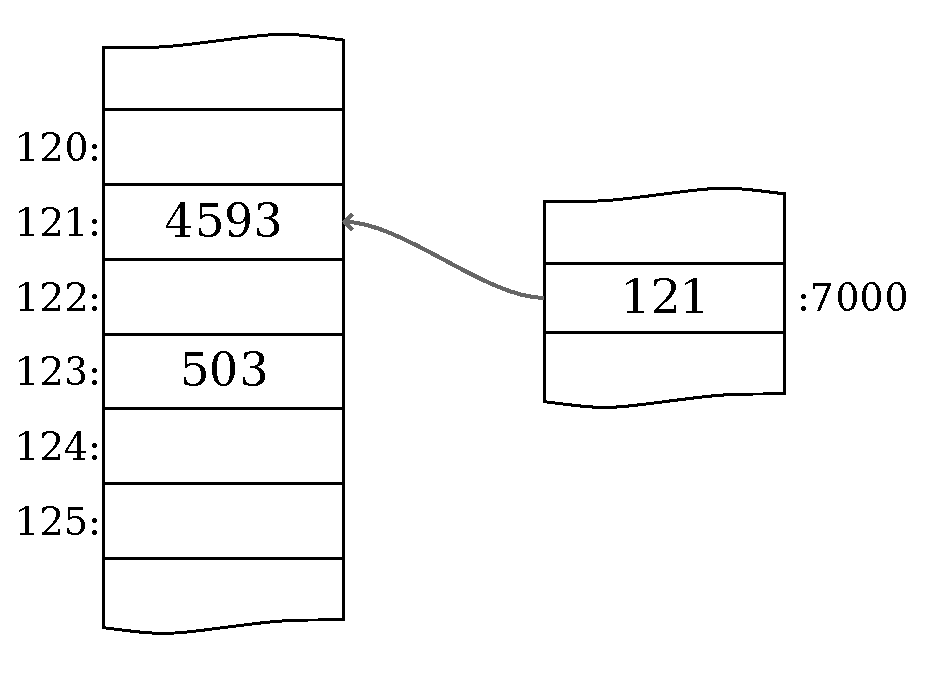
\includegraphics[width=0.6\textwidth]{./Grafiken/Pointer/pointer_stack}
\caption{Der Pointer zeigt auf die Adresse 121} 
\end{figure}


\section{Wie man Pointer benutzt} 

Wie auf dem Bild zu sehen, speichert der Pointer einfach nur eine \emph{Adresse} einer anderen Stelle im Speicher. Verändern wir den Wert auf den der \emph{Pointer} zeigt, ist dies auch für alle anderen \emph{Pointer}, die auf die selbe Stelle zeigen, sichtbar.

In den folgenden Code Beispielen bezeichnen wir die Integer Variable mit \(k\) und den Pointer mit \emph{ptr}.

Zuerst legen wir, wie gewohnt, eine Integer Variable an

\lstinputlisting[firstline=1, lastline=2]{CodeSnippets/Pointer/pointer_commands.c}

Mit dem \& Operator kann man sich die Adresse einer Variable ausgeben lassen.

\lstinputlisting[firstline=4, lastline=5]{CodeSnippets/Pointer/pointer_commands.c}  

Wir möchten, dass unser \emph{Pointer} genau auf die Adresse von \(k\) zeigt. Daher weißen wir dem \emph{Pointer} auch genau diese Adresse zu. Ein \emph{Pointer} muss genau, wie jede andere Variable auch einen Typ haben. Man gibt den Typ der Variable an, auf die der \emph{Pointer} zeigen soll und macht einen * dahinter.

\lstinputlisting[firstline=7, lastline=8]{CodeSnippets/Pointer/pointer_commands.c} 

Wenn wir jetzt den \emph{Pointer} ptr ausgeben lassen, bekommen wir genau die selbe Adresse zurück, die wir bei der Adresse von \(k\) bekommen haben. Diesmal schreiben wir allerdings kein \& Operator vor prt, denn die Adresse ist bereits der \textbf{Wert} von ptr.

\lstinputlisting[firstline=10, lastline=11]{CodeSnippets/Pointer/pointer_commands.c} 

Wenn wir jetzt die Adresse des \emph{Pointers} selbst ausgeben lassen, bekommen wir die \emph{Adresse} des Speichers an dem der \emph{Pointer} selbst gespeichert ist. Wie man an der Grafik sehen kann, ist das die 7000.

\lstinputlisting[firstline=13, lastline=14]{CodeSnippets/Pointer/pointer_commands.c} 

Mit dem *, dem \emph{Dereferenzierungsopterator}, kommt man an den Wert, auf den der \emph{Pointer} zeigt. Schreibt man den * vor eine Variable wird deren Inhalt als Adresse interpretiert, und das Programm schaut nach, was an dieser Stelle steht.

\lstinputlisting[firstline=16, lastline=17]{CodeSnippets/Pointer/pointer_commands.c} 

Wenn dann der Wert von \(k\) verändert wird, ist das auch für den \emph{Pointer} sichtbar. Dieser \textbf{zeigt} ja nur auf diesen Wert.

\lstinputlisting[firstline=19, lastline=22]{CodeSnippets/Pointer/pointer_commands.c} 

Das ganze funktioniert natürlich auch umgekehrt, indem man den Wert über den \emph{Pointer} verändert.

\lstinputlisting[firstline=24, lastline=27]{CodeSnippets/Pointer/pointer_commands.c}



\section{Mehrere Pointer} 

\begin{figure}[h]
\centering
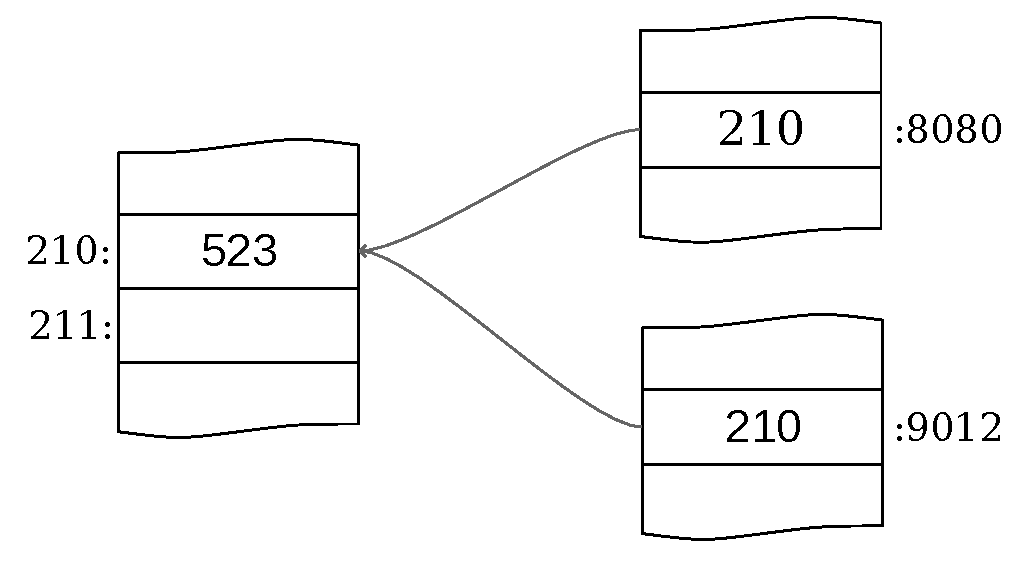
\includegraphics[width=0.6\textwidth]{Grafiken/Pointer/2pointer}
\caption{2 Pointer zeigen auf die selbe Adresse} 
\end{figure}

In diesem Beispiel zeigen zwei \emph{Pointer} auf die selbe \emph{Adresse}. Das heißt man kann über beide auf den Wert in der \emph{Adresse} 210 zugreifen und diesen auch verändern.

\lstinputlisting{CodeSnippets/Pointer/2pointer.c} 



\section{Dereferenzierung}

Nutzt man den \emph{Dereferenzierungsoperator} * auf eine Variable, wird nichts anderes getan als, dass der Wert der Variable als \emph{Adresse} interpretiert wird und dort nachgeschaut wird. 

Den Operator auf einer \emph{Nicht Pointer Variable} aufzurufen, ergibt keinen Sinn, ist aber möglich. Angenommen die Integer Variable \(k\) hat den Wert 145 und man ruft *\(k\) auf, schaut das Programm an die \emph{Adresse} 145 im Speicher. Dort kann alles Mögliche stehen, aber meistens nichts sinnvolles. Im schlimmsten Fall darf man auf diesen Speicher gar nicht zugreifen und das Programm stürzt ab.



\section{Adressarithmetik}

Man kann auch direkt Rechenoperationen auf den Adressen von \emph{Pointern} durchführen. Ein \emph{Pointer} hat genau wie eine Variable einen \emph{Typ} und dieser hat eine Größte in Byte. So hat z.B. ein \emph{Integer} im Normalfall 4 Byte und ein \emph{Character} nur einen Byte.

\lstinputlisting{CodeSnippets/Pointer/pointerarithmetik.c} 

Genau das passiert effektiv bei \emph{Arrays}.


\end{document}